\documentclass[12pt]{scrartcl}
\usepackage[utf8]{inputenc}
\usepackage{hyperref}
\usepackage{booktabs}
\usepackage{caption}
\usepackage{graphicx}

\begin{document}


\title{A Fast Approximation of the Weisfeiler-Lehman Graph Kernel for RDF Data}
\subtitle{Referee report}
\author{
Emilio Cecchini \\ \href{mailto:emilio.cecchini@stud.unifi.it}{emilio.cecchini@stud.unifi.it}
\and
Lorenzo Palloni \\ \href{mailto:lorenzo.palloni@stud.unifi.it}{lorenzo.palloni@stud.unifi.it}
}

\maketitle

\section{Summary}

The goal of this paper is to introduce a faster version of the Weisfeiler-Lehman graph kernel algorithm when applied to Resource Description Framework (RDF) data.

The \textit{Resource Description Framework} (RDF) is the foundation for knowledge representation on the semantic web. A resource is described by a set of \textit{triples} which are of the form \textit{subject-predicate-object}. The entire collection of triples form a graph where the subjects and the objects are the nodes and the predicates are the edges.

The \textit{Weisfeiler-Lehman test} is an algorithm that is used to compute graph isomorphism. The test proceeds in iterations where the key idea is to augment the node labels by the sorted set of node labels of neighbouring nodes, and compress these augmented labels into new, short labels. These steps are then repeated until the node label sets of the two graphs differ, or the number of iterations reaches the prefixed maximum.

The \textit{Weisfeiler-Lehman kernel} is the state-of-the-art for graph kernels. It computes the number of subtrees shared between two graphs by using the Weisfeiler-Lehman test of graph isomorphism.

This paper introduces an approximation of the Weisfeiler-Lehman kernel, which first extracts a set of subgraphs from the entire RDF graph and then the kernels are computed. For each instance a subgraph up to a certain depth is extracted from the RDF dataset and this subgraph is added to a total graph that the extraction algorithm is building. Thus, vertices and edges are only added if they have not been added to the graph already. For each node and edge, together with their labels, their extraction depth is stored. The relabeling process is the same of the standard Weisfeiler-Lehman test with the extension of the labels on the edges. Finally the kernel is computed by counting the number of common labels at each depth.

\section{Evaluation}

In this paper there is no formal theorem or proof. The author states that this kernel yields an approximation of the standard Weisfeiler-Lehman graph kernel, but he never actually gives any formal proof of the accuracy of that approximation. The comparison of the results with the standard Weisfeiler-Lehman graph kernel can be found only in the experiments section. However there is a good explanation on how the complexity of the algorithm is improved with this approximation.

In the first experiment, where a classification on the SWRC ontology \cite{swrc} is performed, the author specify that the \textit{affiliation} relation and its inverse (the \textit{employs} relation) were removed from the dataset for training purposes. We instead discovered that there are two other relationships that must be removed because they link the instances to their corresponding class, these relationships are \textit{member} and \textit{head}. The fact that these two predicates were not removed from the training dataset led to a higher accuracy than the real one.

The plots of the runtime experiments are inverted: the lithogenesis dataset is about ten time larger than the affiliation dataset, but the reported runtimes of the lithogenesis classification are ten smaller than the runtimes of the affiliation prediction.

This paper proposes a new method on computing graph kernels, but it is limited only to RDF data. This method exploits the fact that usually, in the RDF graphs, the extracted sugraphs share many nodes and edges. This fact limits the number of scenarios in which the method is applicable with good results.

The algorithm described in this paper is an approximation of the Weisfeiler-Lehman graph kernel proposed in \cite{wl-kernels}. The approximation algorithm is very similar to the standard one described in \cite{wl-kernels}, the only difference is that the label expansion process is also extended to the edges and the concept of \textit{depth} is introduced in order to have bigger graphs without storing duplicated nodes or edges. This two simple modifications seem to lead to a faster version, but there is not much innovation in this new proposed method.

The proposed kernel method is a tool to perform machine learning algorithms on RDF data. There is a small section in the paper where the author introduces the \textit{Resource Description Framework}, but it is never clearly explained what it means to perform a classification on that kind of data.

During the extraction process of the subgraphs of the instances, the algorithm keeps track of the extraction depth to which each node and edge were extracted. In the paper there is confusion about the order of the index of the depth. In the pseudocode of the algorithm the depth is counted backward, that is the root has index equal to the maximum extraction depth while the leaves of the tree has depth equal to zero. While in the explanation of the algorithm the author describes the process with the indexes inverted.

The datasets used in the experiments are still available online. There is a GitHub repository that contains the source code of the experiments but it is quite old and we were not able to compile and to run it.


\section{Replication of the experiments}

Since we were not able to compile and to run the experiments done by the author, we have implemented a small part of the experiments in order to assess the validity of the results in the paper. We have implemented the standard Weisfeiler-Lehman graph kernel and its approximation proposed in the paper. The source code for the kernels and the experiments are available online \footnote{https://github.com/deeplego/wl-graph-kernels}. We have perfomed a classification on the AIFB dataset \cite{swrc} and the 'Named Rock Units' dataset of the  British Geological Survey. We have used the C-Support Vector Machine algorithm found in the scikit-learn Python package. We have tried to compute the accuracy of the classification with the same method described in the paper, that is a 10-fold cross-validation, however we slightly semplified the process of computing the accuracy of the model in relation to the C parameter of the SVM. We executed a 10-fold cross-validation for each value of C in $\{10^{-3}, 10^{-2}, 10^{-1}, 1, 10^1, 10^2, 10^3\}$ and then we took the best accuracy value. The results of the classifications are reported in the tables below.

\newpage

\begin{center}
\captionof{table}{Affiliation prediction with the standard Weisfeiler-Lehman kernel}
\begin{tabular}{ccccc}
\toprule
 depth & iterations &  accuracy &        f1 &      C \\
\midrule
1 & 0 &  0.842337 &  0.772552 &  100.0 \\
  & 2 &  0.836782 &  0.755789 &  100.0 \\
  & 4 &  0.836782 &  0.755789 &  100.0 \\
  & 6 &  0.836782 &  0.755789 &  100.0 \\
\hline
2 & 0 &  0.892516 &  0.836455 &  100.0 \\
  & 2 &  0.826180 &  0.742251 &  100.0 \\
  & 4 &  0.774069 &  0.618519 &  100.0 \\
  & 6 &  0.740048 &  0.568392 &  100.0 \\
\hline
3 & 0 &  0.892591 &  0.850147 &  100.0 \\
  & 2 &  0.897779 &  0.848919 &  100.0 \\
  & 4 &  0.909258 &  0.860964 &  100.0 \\
  & 6 &  0.881044 &  0.796105 &  100.0 \\
\bottomrule
\end{tabular}
\end{center}

\begin{center}
\captionof{table}{Affiliation prediction with the Weisfeiler-Lehman for RDF}
\begin{tabular}{ccccc}
\toprule
depth & iterations & accuracy & f1 & C \\
\midrule
1 & 0 &  0.881955 &  0.795756 &  100.0 \\
  & 2 &  0.881955 &  0.795756 &  100.0 \\
  & 4 &  0.881955 &  0.795756 &  100.0 \\
  & 6 &  0.881955 &  0.795756 &  100.0 \\
\hline
2 & 0 &  0.892114 &  0.826007 &  100.0 \\
  & 2 &  0.880057 &  0.812488 &  100.0 \\
  & 4 &  0.874501 &  0.803701 &  100.0 \\
  & 6 &  0.874501 &  0.800821 &  100.0 \\
\hline
3 & 0 &  0.879579 &  0.812187 &  100.0 \\
  & 2 &  0.913751 &  0.867388 &  100.0 \\
  & 4 &  0.908196 &  0.863829 &  100.0 \\
  & 6 &  0.908196 &  0.863829 &  100.0 \\
\bottomrule
\end{tabular}
\end{center}

\newpage

\begin{center}
\captionof{table}{Lithogenesis prediction with the standard Weisfeiler-Lehman kernel}
\begin{tabular}{ccccc}
\toprule
depth & iterations &  accuracy &        f1 &      C \\
\midrule
1 & 0 &  0.802679 &  0.774383 &   10.0 \\
  & 2 &  0.796429 &  0.768842 &   10.0 \\
  & 4 &  0.796429 &  0.768842 &   10.0 \\
  & 6 &  0.796429 &  0.768842 &   10.0 \\
\hline
2 & 0 &  0.891964 &  0.877311 &  100.0 \\
  & 2 &  0.892857 &  0.874092 &    1.0 \\
  & 4 &  0.873214 &  0.854485 &    1.0 \\
  & 6 &  0.865179 &  0.841353 &    1.0 \\
\hline
3 & 0 &  0.883929 &  0.871406 &  100.0 \\
  & 2 &  0.913393 &  0.898291 &    1.0 \\
  & 4 &  0.906250 &  0.890922 &    1.0 \\
  & 6 &  0.906250 &  0.890922 &    1.0 \\
\bottomrule
\end{tabular}
\end{center}

\begin{center}
\captionof{table}{Lithogenesis prediction with the Weisfeiler-Lehman kernel for RDF}
\begin{tabular}{ccccc}
\toprule
depth & iterations & accuracy & f1 & C \\
\midrule
1 & 0 &  0.795536 &  0.763739 &   10.0 \\
  & 2 &  0.795536 &  0.763739 &   10.0 \\
  & 4 &  0.795536 &  0.763739 &   10.0 \\
  & 6 &  0.795536 &  0.763739 &   10.0 \\
\hline
2 & 0 &  0.906250 &  0.891229 &  100.0 \\
  & 2 &  0.892857 &  0.874092 &    1.0 \\
  & 4 &  0.892857 &  0.874092 &    1.0 \\
  & 6 &  0.885714 &  0.866606 &    1.0 \\
\hline
3 & 0 &  0.891071 &  0.875862 &  100.0 \\
  & 2 &  0.891964 &  0.873422 &    1.0 \\
  & 4 &  0.906250 &  0.890104 &    1.0 \\
  & 6 &  0.907143 &  0.888829 &    1.0 \\
\bottomrule
\end{tabular}
\end{center}

The accuracy values are almost the same as those reported in the paper. There is not much difference between the standard Weisfeiler-Lehman algorithm and its approximation in terms of accuracy.

We have also replicated the experiment of the affiliation prediction where all the labels were removed from the graph. The results are given in the two table belows. This is the best scenario for the Weisfeiler-Lehman kernel for RDF data. As reported in the paper, these results are very similar to the performance on labeled graphs.

\newpage

\begin{center}
\captionof{table}{Affiliation prediction with the standard Weisfeiler-Lehman kernel with all labels removed}
\begin{tabular}{ccccc}
\toprule
depth & iterations & accuracy & f1 & C \\
\midrule
1 & 0 &  0.322153 &  0.194477 &  100.0 \\
  & 2 &  0.530111 &  0.348672 &   10.0 \\
  & 4 &  0.530111 &  0.347049 &   10.0 \\
  & 6 &  0.530111 &  0.347049 &   10.0 \\
\hline
2 & 0 &  0.564547 &  0.355253 &   10.0 \\
  & 2 &  0.503724 &  0.343148 &    1.0 \\
  & 4 &  0.481437 &  0.392366 &  100.0 \\
  & 6 &  0.502999 &  0.383461 &    1.0 \\
\hline
3 & 0 &  0.491697 &  0.343404 &  100.0 \\
  & 2 &  0.641333 &  0.527556 &  100.0 \\
  & 4 &  0.724551 &  0.602677 &   10.0 \\
  & 6 &  0.713474 &  0.557335 &  100.0 \\
\bottomrule
\end{tabular}
\end{center}

\begin{center}
\captionof{table}{Affiliation prediction with the Weisfeiler-Lehman kernel for RDF with all labels removed}
\begin{tabular}{ccccc}
\toprule
depth & iterations & accuracy & f1 & C \\
\midrule
1 & 0 &  0.524847 &  0.305547 &  100.0 \\
  & 2 &  0.647536 &  0.566394 &  100.0 \\
  & 4 &  0.670780 &  0.591060 &  100.0 \\
  & 6 &  0.677030 &  0.594329 &  100.0 \\
\hline
2 & 0 &  0.565936 &  0.340732 &   10.0 \\
  & 2 &  0.681422 &  0.622212 &  100.0 \\
  & 4 &  0.740048 &  0.663960 &  100.0 \\
  & 6 &  0.762597 &  0.688069 &  100.0 \\
\hline
3 & 0 &  0.407394 &  0.293320 &    1.0 \\
  & 2 &  0.898914 &  0.861681 &  100.0 \\
  & 4 &  0.892079 &  0.854304 &  100.0 \\
  & 6 &  0.893066 &  0.851358 &   10.0 \\
\bottomrule
\end{tabular}
\end{center}

\newpage

Since this new method is supposed to be faster, we also replicated the experiments on the runtimes. The Weisfeiler-Lehman for RDF method is slightly faster then the regular one, but we were not able to see such a good improvements in the runtime as reported in the paper.

\begin{center}
\begin{figure}[h]
\caption{Runtimes of the two kernels on the affiliation dataset}
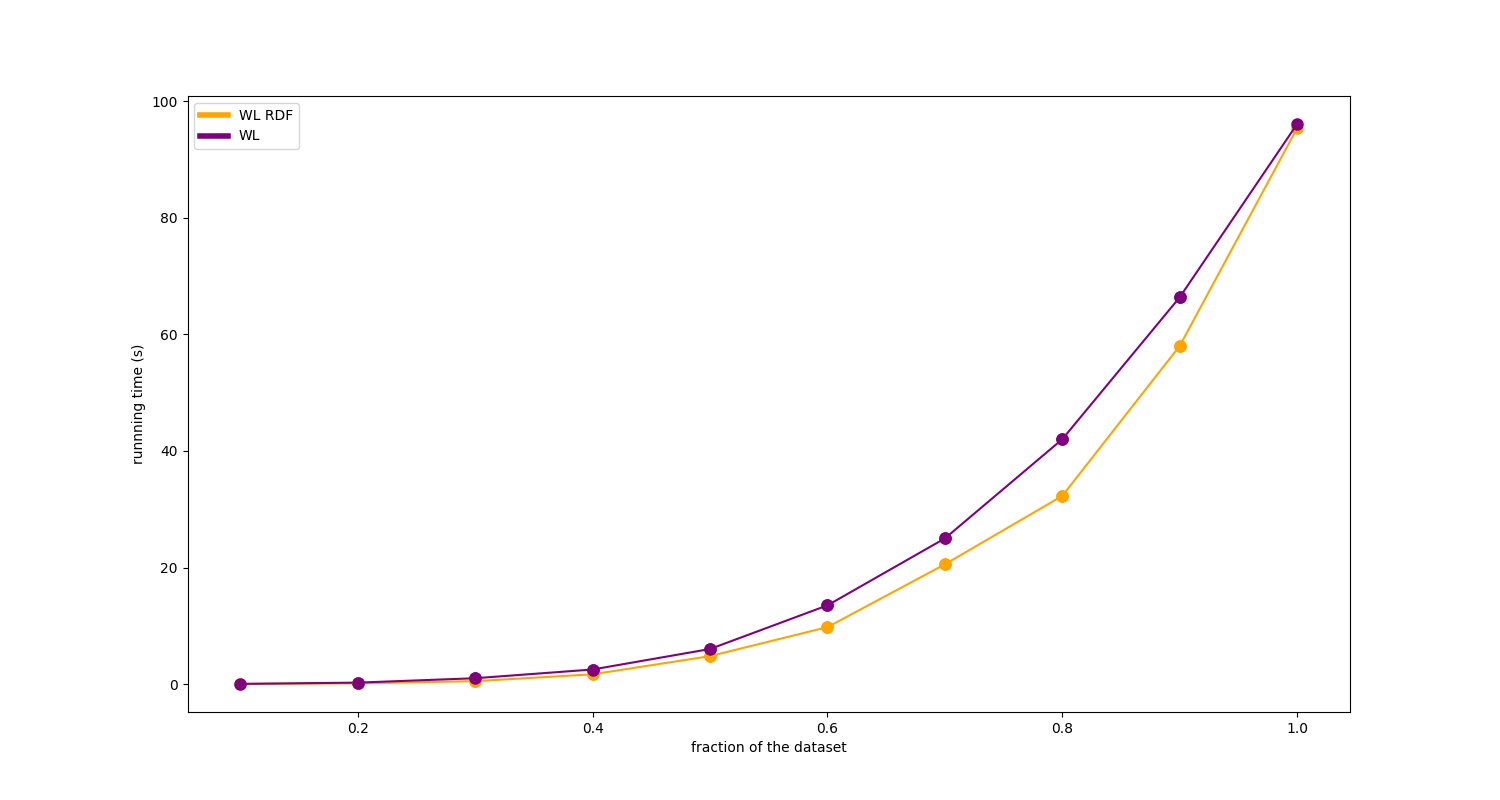
\includegraphics[width=\textwidth]{img/affiliation_timing.png}
\end{figure}
\end{center}

\begin{center}
\begin{figure}[h]
\caption{Runtimes of the two kernels on the lithogenesis dataset}
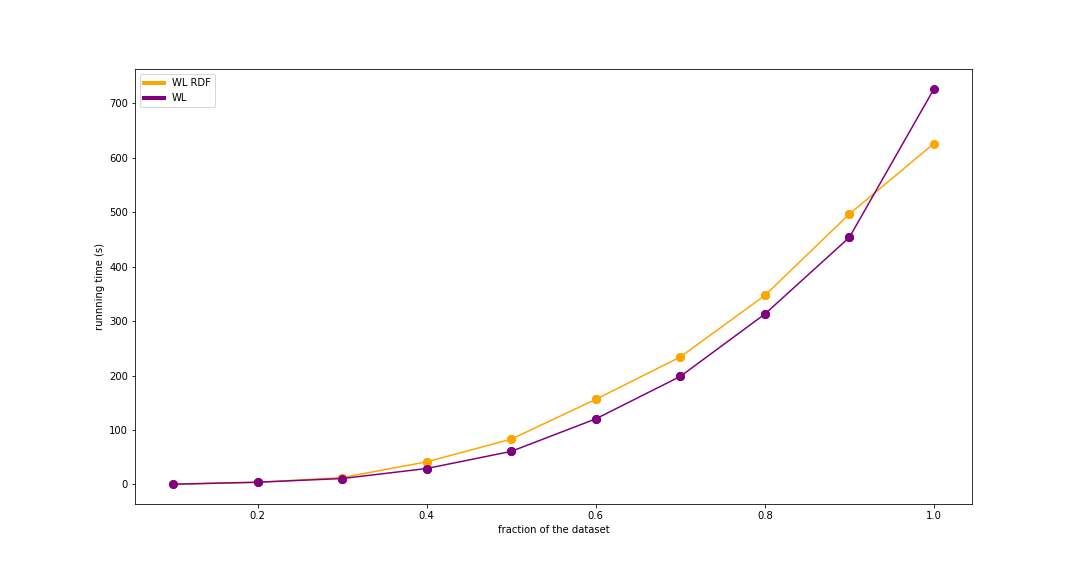
\includegraphics[width=\textwidth]{img/lithogenesis_timing.png}
\end{figure}
\end{center}

\newpage

\begin{thebibliography}{9}

\bibitem{lamport94}
    Vries Gerben Klaas Dirk,
    A Fast Approximation of the Weisfeiler-Lehman Graph Kernel for RDF Data,
    2013

\bibitem{swrc}
    Sure, Y., Bloehdorn, S., Haase, P., Hartmann, J., Oberle, D.,
    The swrc ontology - semantic web for research communities.
    Volume 3803 of LNCS., Covilha,
    Portugal, Springer (Dezember 2005) 218 – 231

\bibitem{wl-kernels}
    Shervashidze, N., Schweitzer, P., van Leeuwen, E.J., Mehlhorn, K., Borgwardt, K.M.
    Weisfeiler-lehman graph kernels,
    2011

\end{thebibliography}

\end{document}
